
% Programming/Coding Assignment
% LaTeX Template
%
% This template has been downloaded from:
% http://www.latextemplates.com
%
% Original author:
% Ted Pavlic (http://www.tedpavlic.com)
%
% Note:
% The \lipsum[#] commands throughout this template generate dummy text
% to fill the template out. These commands should all be removed when 
% writing assignment content.
%
% This template uses a Perl script as an example snippet of code, most other
% languages are also usable. Configure them in the "CODE INCLUSION 
% CONFIGURATION" section.
%
%%%%%%%%%%%%%%%%%%%%%%%%%%%%%%%%%%%%%%%%%

%----------------------------------------------------------------------------------------
%   PACKAGES AND OTHER DOCUMENT CONFIGURATIONS
%----------------------------------------------------------------------------------------

\documentclass{article}

\usepackage{fancyhdr} % Required for custom headers
\usepackage{lastpage} % Required to determine the last page for the footer
\usepackage{extramarks} % Required for headers and footers
\usepackage[usenames,dvipsnames]{color} % Required for custom colors
\usepackage{graphicx} % Required to insert images
\usepackage{listings} % Required for insertion of code
\usepackage{courier} % Required for the courier font
\usepackage{lipsum} % Used for inserting dummy 'Lorem ipsum' text into the template
\usepackage{fullpage,amsthm,amsfonts,amssymb,epsfig,amsmath}

% Margins
\topmargin=-0.45in
\evensidemargin=0in
\oddsidemargin=0in
\textwidth=6.5in
\textheight=9.0in
\headsep=0.25in

\linespread{1.1} % Line spacing

% Set up the header and footer
\pagestyle{fancy}
\lhead{\hmwkAuthorName} % Top left header
\chead{\hmwkClass\ (\hmwkClassInstructor\ \hmwkClassTime): \hmwkTitle} % Top center head
\rhead{\firstxmark} % Top right header
\lfoot{\lastxmark} % Bottom left footer
\cfoot{} % Bottom center footer
\rfoot{Page\ \thepage\ of\ \protect\pageref{LastPage}} % Bottom right footer
\renewcommand\headrulewidth{0.4pt} % Size of the header rule
\renewcommand\footrulewidth{0.4pt} % Size of the footer rule
\newcommand{\tab}{\hspace*{3em}}

\setlength\parindent{0pt} % Removes all indentation from paragraphs

%----------------------------------------------------------------------------------------
%   CODE INCLUSION CONFIGURATION
%----------------------------------------------------------------------------------------

\definecolor{MyDarkGreen}{rgb}{0.0,0.4,0.0} % This is the color used for comments
\lstloadlanguages{Perl} % Load Perl syntax for listings, for a list of other languages supported see: ftp://ftp.tex.ac.uk/tex-archive/macros/latex/contrib/listings/listings.pdf
\lstset{language=Perl, % Use Perl in this example
        frame=single, % Single frame around code
        basicstyle=\small\ttfamily, % Use small true type font
        keywordstyle=[1]\color{Blue}\bf, % Perl functions bold and blue
        keywordstyle=[2]\color{Purple}, % Perl function arguments purple
        keywordstyle=[3]\color{Blue}\underbar, % Custom functions underlined and blue
        identifierstyle=, % Nothing special about identifiers                                         
        commentstyle=\usefont{T1}{pcr}{m}{sl}\color{MyDarkGreen}\small, % Comments small dark green courier font
        stringstyle=\color{Purple}, % Strings are purple
        showstringspaces=false, % Don't put marks in string spaces
        tabsize=5, % 5 spaces per tab
        %
        % Put standard Perl functions not included in the default language here
        morekeywords={rand},
        %
        % Put Perl function parameters here
        morekeywords=[2]{on, off, interp},
        %
        % Put user defined functions here
        morekeywords=[3]{test},
        %
        morecomment=[l][\color{Blue}]{...}, % Line continuation (...) like blue comment
        numbers=left, % Line numbers on left
        firstnumber=1, % Line numbers start with line 1
        numberstyle=\tiny\color{Blue}, % Line numbers are blue and small
        stepnumber=5 % Line numbers go in steps of 5
}

% Creates a new command to include a perl script, the first parameter is the filename of the script (without .pl), the second parameter is the caption
\newcommand{\perlscript}[2]{
\begin{itemize}
\item[]\lstinputlisting[caption=#2,label=#1]{#1.pl}
\end{itemize}
}

%----------------------------------------------------------------------------------------
%   DOCUMENT STRUCTURE COMMANDS
%   Skip this unless you know what you're doing
%----------------------------------------------------------------------------------------

% Header and footer for when a page split occurs within a problem environment
\newcommand{\enterProblemHeader}[1]{
\nobreak\extramarks{#1}{#1 continued on next page\ldots}\nobreak
\nobreak\extramarks{#1 (continued)}{#1 continued on next page\ldots}\nobreak
}

% Header and footer for when a page split occurs between problem environments
\newcommand{\exitProblemHeader}[1]{
\nobreak\extramarks{#1 (continued)}{#1 continued on next page\ldots}\nobreak
\nobreak\extramarks{#1}{}\nobreak
}

\setcounter{secnumdepth}{0} % Removes default section numbers
\newcounter{homeworkProblemCounter} % Creates a counter to keep track of the number of problems

\newcommand{\homeworkProblemName}{}
\newenvironment{homeworkProblem}[1][Problem \arabic{homeworkProblemCounter}]{ % Makes a new environment called homeworkProblem which takes 1 argument (custom name) but the default is "Problem #"
\stepcounter{homeworkProblemCounter} % Increase counter for number of problems
\renewcommand{\homeworkProblemName}{#1} % Assign \homeworkProblemName the name of the problem
\section{\homeworkProblemName} % Make a section in the document with the custom problem count
\enterProblemHeader{\homeworkProblemName} % Header and footer within the environment
}{
\exitProblemHeader{\homeworkProblemName} % Header and footer after the environment
}

\newcommand{\problemAnswer}[1]{ % Defines the problem answer command with the content as the only argument
\noindent\framebox[\columnwidth][c]{\begin{minipage}{0.98\columnwidth}#1\end{minipage}} % Makes the box around the problem answer and puts the content inside
}

\newcommand{\homeworkSectionName}{}
\newenvironment{homeworkSection}[1]{ % New environment for sections within homework problems, takes 1 argument - the name of the section
\renewcommand{\homeworkSectionName}{#1} % Assign \homeworkSectionName to the name of the section from the environment argument
\subsection{\homeworkSectionName} % Make a subsection with the custom name of the subsection
\enterProblemHeader{\homeworkProblemName} % Header and footer within the environment
}{
\enterProblemHeader{\homeworkProblemName} % Header and footer after the environment
}

%----------------------------------------------------------------------------------------
%   NAME AND CLASS SECTION
%----------------------------------------------------------------------------------------

\newcommand{\hmwkTitle}{Homework\ \#4} % Assignment title
\newcommand{\hmwkDueDate}{Tuesday,\ April\ 28st,\ 2015} % Due date
\newcommand{\hmwkClass}{CMPS\ 102} % Course/class
\newcommand{\hmwkClassTime}{4:00pm} % Class/lecture time
\newcommand{\hmwkClassInstructor}{Warmuth} % Teacher/lecturer
\newcommand{\hmwkAuthorName}{John Allard \ 1437547} % Your name


%----------------------------------------------------------------------------------------
%----------------------------------------------------------------------------------------
%   USER SETTINGS
%----------------------------------------------------------------------------------------
%----------------------------------------------------------------------------------------
\usepackage{mathtools}
\DeclarePairedDelimiter\ceil{\lceil}{\rceil}
\DeclarePairedDelimiter\floor{\lfloor}{\rfloor}



%----------------------------------------------------------------------------------------
%   TITLE PAGE
%----------------------------------------------------------------------------------------

\title{
\vspace{2in}
\textmd{\textbf{\hmwkClass:\ \hmwkTitle}}\\
\normalsize\vspace{0.1in}\small{Due\ on\ \hmwkDueDate}\\
\vspace{0.1in}\large{\textit{}}
\vspace{3in}
}

\author{\textbf{\hmwkAuthorName}}
\date{} % Insert date here if you want it to appear below your name

%----------------------------------------------------------------------------------------

\begin{document}

\maketitle

%----------------------------------------------------------------------------------------
%   TABLE OF CONTENTS
%----------------------------------------------------------------------------------------

%\setcounter{tocdepth}{1} % Uncomment this line if you don't want subsections listed in the ToC

% \tableofcontents
\newpage





%----------------------------------------------------------------------------------------
%   PROBLEM 1
%----------------------------------------------------------------------------------------

% To have just one problem per page, simply put a \clearpage after each problem

\begin{homeworkProblem}

Suppose Dijkstra's algorithm is run on the following graph, starting at node A. \\

\begin{center}
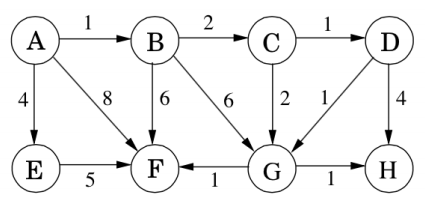
\includegraphics[width=3in]{DPV41.PNG}
\end{center}

\begin{enumerate}

\item Draw a table showing the intermediate distance values of all the nodes at each iteration of the algorithm. \\    

% \begin{tabular}{|c|c|c|c|c|c|c|c|c|} \hline
%        &   a   &   b   &   c   &   d   &   e   &   f   &   g   &   h   \\ \hline
%    a   &   0   &   6   &   .   &   .   &   1   &   .   &   .   &   .   \\ \hline
%    b   &   6   &   0   &   5   &   .   &   2   &   2   &   .   &   .   \\ \hline
%    c   &   .   &   5   &   0   &   6   &   .   &   5   &   4   &   .   \\ \hline
%    d   &   .   &   .   &   6   &   0   &   .   &   .   &   5   &   7   \\ \hline
%    e   &   1   &   2   &   .   &   .   &   0   &   1   &   .   &   .   \\ \hline
%    f   &   .   &   2   &   5   &   .   &   1   &   0   &   3   &   .   \\ \hline
%    g   &   .   &   .   &   4   &   5   &   .   &   3   &   0   &   3   \\ \hline
%    h   &   .   &   .   &   .   &   7   &   .   &   .   &   3   &   3   \\ \hline
% \end{tabular} 

The table below shows each iteration as a row, with later iterations being below earlier iterations. The numbers in each table section represent the shortest distance knows from the source (vertex A) to the vertex corresponding to that column during the iteration given by the row number. The distances to A are always zero because A is the source. For brevity, I use a `.' instead of an $\infty$ to represent infinite distances.

\begin{tabular}{|c|c|c|c|c|c|c|c|c|} \hline
 d(x) &   a   &   b   &   c   &   d   &   e   &   f   &   g   &   h   \\ \hline
      &   0   &   .   &   .   &   .   &   .   &   .   &   .   &   .   \\ \hline
      &   0   &   1   &   .   &   .   &   4   &   8   &   .   &   .   \\ \hline
      &   0   &   1   &   3   &   .   &   4   &   7   &   7   &   .   \\ \hline
      &   0   &   1   &   3   &   4   &   4   &   7   &   5   &   4   \\ \hline
      &   0   &   1   &   3   &   4   &   4   &   7   &   5   &   4   \\ \hline
      &   0   &   1   &   3   &   4   &   4   &   7   &   5   &   4   \\ \hline
      &   0   &   1   &   3   &   4   &   4   &   6   &   5   &   4   \\ \hline
      &   0   &   1   &   3   &   4   &   4   &   6   &   5   &   4   \\ \hline
\end{tabular} 


\item Show the final shortest-path tree. \\

\begin{center}
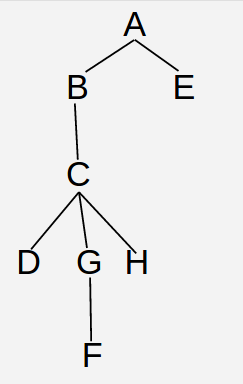
\includegraphics[width=2in]{sssp_tree.png}
\end{center}


\end{enumerate}


\end{homeworkProblem}






%----------------------------------------------------------------------------------------
%   PROBLEM 2
%----------------------------------------------------------------------------------------

\begin{homeworkProblem}

Consider the following graph \\

\begin{center}
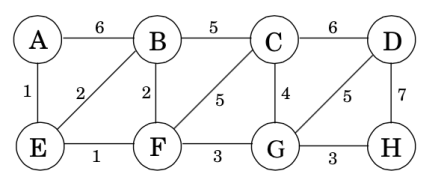
\includegraphics[width=3in]{DPV51.PNG}
\end{center}

\begin{enumerate}

\item What is the cost of it's minimum spanning tree? \\ The total cost of the minimum spanning tree is 14, it consists of the following edges :
$$ [(A,E,1), (E,B,2), (E,F,1), (F,G,3), (G,C,4), (G,H,3)] $$

\item How many minimum spanning trees does it have? \\ By Caley's theorem, there are $n^{n-2}$ spanning trees, given that $n=8$, the number of spanning trees is $8^6=262144$.

\item Suppose Kruskals algortithm is run on this graph. In what order are the edges added to the MST? For each edge in this sequence give a cut that justifies its addition. \\

Below is a table that answers the question above. It shows the steps of the algorithm going down the table, with the groups
of vertices being shown in the other columns. Notice they all start out as singletons before being formed into a single tree.
This example is odd in that no other components of size greater than one were created, all iterations consisted of adding a singleton to the current tree, which does not have to happen with Kruskal's algorithm. \\
\begin{tabular}{|c|c|c|c|c|c|c|c|c|} \hline
iteration & A & B & C & D & E & F & G & H \\ \hline
        1 & AE & B & C & D &  & F & G & H \\ \hline
        2 & AEF & B & C & D &  &  & G & H \\ \hline
        3 & AEFB &  & C & D &  &  & G & H \\ \hline
        4 & AEFBG &  & C & D &  &  &  & H \\ \hline
        5 & AEFBGH &  & C & D &  &  &  &  \\ \hline
        6 & AEFBGHC &  &  & D &  &  &  &  \\ \hline
        7 & AEFBGHCD &  &  &  &  &  &  &  \\ \hline 
\end{tabular}

\end{enumerate}

\end{homeworkProblem}





%----------------------------------------------------------------------------------------
%   PROBLEM 3
%----------------------------------------------------------------------------------------
\begin{homeworkProblem}
You are given an unbounded array $A[1],A[2],A[3], \ldots]$ containing
distinct integers sorted in ascending order. Describe an
efficient algorithm that takes an integer $k$ as input and
finds out whether $k$ is in the array in time
$O(\log p)$ time where $p$ is the number of integers in the
array that are strictly less than $k$. \\

Since the required runtime is $O(log(p))$, I know I am going to have to shrink the search space by a constant factor for each iteration. This will result in an exponentially-conquering search of the space, which will reduce the run-time needed to process $n$ elements from linear to logarithmic. To do this, I will use a technique inspired by the exponential backoff algorithm. Instead of looking at each element in the array starting from the first element and continuing until we find the one we're looking for, I will look at every $2^n$th item for $n \in \mathbb{n}$. Once I find an element larger than the desired element, I can simply perform a binary search in between the last two elements I have looked at. Since the entire array is ordered, binary search will work correctly and the element will be found. The algorithm is given below and they are discussed in detail below that. : \\ 

\problemAnswer{
    \texttt{// A = unbounded, sorted array on integers starting at index 1} \\
    \texttt{// x is the element we are searching A for} \\
    \texttt{ 1.} \texttt{ findx(A, x) : } \\
    \texttt{ 2.} \texttt{ \tab ind = 1} \\
    \texttt{ 3.} \texttt{ \tab if x = A[ind] : // special case, first item in array} \\
    \texttt{ 4.} \texttt{ \tab \tab return true} \\
    \texttt{ 5.} \texttt{ \tab else if x < A[ind] : // if its less than element \#1 it can't exist} \\
    \texttt{ 6.} \texttt{ \tab \tab return false} \\
    \texttt{ 7.} \texttt{ \tab while A[ind] <= x : // while we haven't passed p} \\
    \texttt{ 8.} \texttt{ \tab \tab ind = ind*2 // double the index value} \\
    \texttt{ 9.} \texttt{ \tab result = BinarySearch(A, x, ind/2, ind) } \\
    \texttt{ 10.} \texttt{ \tab if result == -1 : // wasn't found in the sub-array} \\
    \texttt{ 11.} \texttt{ \tab \tab return false} \\
    \texttt{ 12.} \texttt{ \tab else : } \\
    \texttt{ 13.} \texttt{ \tab \tab return true // was found in the sub-array} \\

    \texttt{// A = sorted array, x is the element we are searching A for} \\
    \texttt{// l is left index of subarray to search, r is right index } \\
    \texttt{// returns index of x if found, -1 otherwise } \\
    \texttt{ 1.} \texttt{ BinarySearch(A, x, l, r) : } \\
    \texttt{ 2.} \texttt{ \tab if r == l :} \\
    \texttt{ 3.} \texttt{ \tab \tab if x == A[r] : } \\
    \texttt{ 4.} \texttt{ \tab \tab \tab return r} \\
    \texttt{ 5.} \texttt{ \tab \tab else : } \\
    \texttt{ 6.} \texttt{ \tab \tab \tab return -1} \\
    \texttt{ 7.} \texttt{ \tab ind =  (r+l)/2} \\
    \texttt{ 8.} \texttt{ \tab if x == A[ind]  : // we found it} \\
    \texttt{ 9.} \texttt{ \tab \tab return ind} \\
    \texttt{ 10.} \texttt{ \tab else if x < A[ind]  : // while we haven't passed p} \\
    \texttt{ 11.} \texttt{ \tab \tab return BinarySearch(A, x, l, ind)} \\
    \texttt{ 12.} \texttt{ \tab else if x > A[ind]  : // while we haven't passed p} \\
    \texttt{ 13.} \texttt{ \tab \tab return BinarySearch(A, x, ind, r)} \\ 
}

I've broken up my implementation into two main parts. The first part scans exponentially from the beginning of the array until it finds an element bigger than $x$, the element we are looking for. At this point, it knows that if the element does exist, it must exist in between the current value which is bigger than $x$ and the last value it looked at which was smaller than $x$. Because the algorithm now knows which two indices the element must exist between (if it exists at all), we can defer the rest of the work to a simple binary search over the sub-array. If the binary search returns an index value, we now know the element exists and so we return true. If BinarySearch returns -1, then we know it wasn't in the subarray and thus doesn't exist at all in the full array. Proofs of correctness and run-tme are given below. \\

\textbf{Proof of Correctness} : \\
The correctness of this algorithm relies on the fact that the elements in the array are sorted in ascending order. Normally, given a sorted array, we would just perform a binary search to locate an element. That of course does not work for this problem because the array is unbounded, but we can reduce this problem to one of binary search with some trickery. The trick is, if we can find two elements, one of which is greater than the item we are looking for and the other of which is smaller, we can reduce this problem to a problem of performing a binary search over the subarray between those two elements. This is enumerated below. \\
Proof : The following properties are used in the proof. \\
\begin{enumerate}
\item Let's say we are looking for an element $x$ in a sorted array $A$. If we examine an element of $A$ and notice it is smaller than $x$, than $x$ must either be further along in the array or it must not exist in the array at all. This is obvious from the properties of a sorted array. \\
\item Likewise, if we're looking for an element $x$ in a sorted array $A$, and we examine an arbitrary element of $A$ and notice it is bigger than $x$, this means that $x$ must either be earlier in the array or not exist at all.  \\
\end{enumerate}

This algorithm is called on an array $A$ and with a value $x$ that we are looking for. It starts by examining the first element in $A$, if it is $x$ then we go ahead and return true. If the element is greater than $x$, we know that $x$ can't exist in the array so we go ahead and return false. Those are the two special cases of this algorithm, the general case of the algorithm in handled next. We start by doubling the index, from 1 to 2. If the $A[2]$ element is greater than $x$, we exit the loop. If it less than $x$, we double the index and repeat the loop. This process of querying and doubling the qqury index repeats until we find some element greater than $x$, which because this is an unbounded increasing array and $x$ is finite must eventually happen. When this does happen we exit the loop. \\
When the loop is exited, we have the index of the first element we have come across that is bigger than $x$. By (2) above, this means that $x$ must either occur earlier in the array or it doesn't exist at all. Likewise, because in the previous iteration we examined the element $A[ind/2]$ and found that element to be less than $x$, by (1) above we know that $x$ must exist at an index after $ind/2$ or it doesn't exist at all. Combining these two facts together means that $x$ must either be between the indices $ind/2$ and $ind$ in $A$, or it doens't exist at all. Thus we know we have reduced the search space of $A$ to a finite number of elements that, if $x$ exists, it must be apart of. This sets us up perfectly for binary search on the subarray $A[ind/2, ind]$, which is called on line 9 of the $findx$ function given above. This binary search now looks for the element $x$, returning its index if it is found and -1 otherwise. If it returns -1, we return false because this means $x$ doesn't exist in the subarray and thus does not exist in $A$ at all, or it is found and its index is returned, in which case we return true.  The correctness of this algorithm depends on the correctness of binary search, which I'm assuming I don't have to prove. /// \\

\textbf{Proof of Run-time Complexity} : \\
The algorithm is required to run in $O(log(p))$, where $p$ is the number of elements in $A$ that are strictly less than the item we are searching for. Because this algorithm consists of two components which are executed in sequence, I will prove that their individual run-times are individually $O(log(p))$, which means that when run back-to-back their total run-time will also be $O(log(p))$. The first algorithm to be proved is the one that finds an element greater than the one we are looking for by checking an exponentially increasing index value in the array. For this I will use a direct proof. \\
Let $x$ be an element you are searching for in a sorted, unbounded array $A$. Let $p$ denote the number of elements in $A$ with values strictly less than $x$. If $x$ exists in $A$, it must be at index $p+1$, given the definition of $p$. This menas our algorithm needs to query an element at an index greater than or equal to $p+1$ in order to find an element that is greater than $x$. The algorithm starts searching at index 1, and doubles the index value before each subsequent query into the array. The number of operations to find an element larger than $x$ is given below :
$$2^k = p+1$$
$$k = \lg(p+1)$$
$$k = \lg(p+1) \leq \lg(p)+1$$
$$k \leq \lg(p)+1$$
$$k = O(log(p))$$
Thus $k$, the number of array queries needed to get to index $p+1$ which contains an element greater than $x$ is $O(log(p))$, as required for the proof. \\

After we have found an element which is greater than $x$, we perform a binary search over a sub-array of $A$. Given that the element larger than $x$ is at index $j$, we now call binary search on the subarray $A[j/2, j]$, inclusive of the end elements. Since we doubled our search index every iteration, and we stopped on the first element greater than $x$ that we found, we know that $j$ is no larger than $2p$, otherwise we would have found an element larger than $x$ during the last iteration. We also know that $j/2 \geq 1$, since all index values we use are positive. This means that BinarySearch will be called on a subarray of size at-most $2p-1$. BinarySearch is logarithmic in the number of elements, so the run-time is $O(log(2p-1))$, which  is of course $O(log(p))$. \\

Because both the algorithm to find an element larger than $x$ and the BinarySearch algorithm to actually find $x$ in a sub-array both run in time $O(log(p))$, the two run in sequence will run in time $O(log(p))+O(log(p))$, which is of course just $O(log(p))$. /// \\

\end{homeworkProblem}





%----------------------------------------------------------------------------------------
%   PROBLEM 4
%----------------------------------------------------------------------------------------
\begin{homeworkProblem}

We define an array $A$ of $n$ objects has a \emph{dominant} object if at least $\lfloor n/2 \rfloor+1$ entries of $A$ are identical. Our goal is to design an efficient algorithm to tell whether the array has a dominant object, and, if so, to find that object. Our only access to $A$ is by making a \textit{query} asking whether $A[i] = A[j]$ for any two $i,j \in \{ 1, 2, \ldots, n \}$. 
\begin{enumerate}
\item[\textbf{(a)}] Design an algorithm to solve this problem with $O(n \log n)$ queries. (\textbf{Hint:} Split the array $A$ into two arrays of half the size.)
\item[\textbf{(b)}] Design an algorithm to solve this problem with $O(n)$ queries. (\textbf{Hint:} Don't Split. Pair up the elements arbitrarily and get rid of as many as you can, repeatedly.)
\end{enumerate}

\end{homeworkProblem}






%----------------------------------------------------------------------------------------
%   PROBLEM 5
%----------------------------------------------------------------------------------------
\begin{homeworkProblem}

KT, problem 17, p 197.)\\
Consider the following variation on the Interval Scheduling Problem.You have a processor that can operate 24 hours a day, every day. People submit requests to run \textit{daily jobs} on the processor. Each such job comes with a \textit{start time} and an \textit{end time}; if the job is accepted to run on the processor, it must run continuously, every day, for the period between its start and end times. (Note that certain jobs can begin before midnight and end after midnight; this makes for a type of situation different from what we saw in the Interval Scheduling Problem.)\\

Given a list of $n$ such jobs, your goal is to accept as many jobs as possible (regardless of their length), subject to the constraint that the processor can run at most one job at any given point in time. Provide an algorithm to do this with a running time that is polynomial in $n$. You may assume for simplicity that no two jobs have the same start or end times.\\

\textbf{Example.} Consider the following four jobs, specified by (\textit{start-time, end- time}) pairs.\\
\begin{displaymath}
\text{(6 PM, 6 AM), (9 PM, 4 AM), (3 AM, 2 PM), (1 PM, 7 PM)}
\end{displaymath}

The optimal solution would be to pick the two jobs (9 P.M., 4 A.M.) and (1 P.M., 7 P.M.), which can be scheduled without overlapping.

\end{homeworkProblem}






%----------------------------------------------------------------------------------------
%   PROBLEM 6
%----------------------------------------------------------------------------------------
\begin{homeworkProblem}

(KT, problem 4, p 190)\\
Sorry too long to retype. Use a greedy algorithm.
Reason your time bound as well as correctness.

\end{homeworkProblem}





%----------------------------------------------------------------------------------------
%   PROBLEM 7 EC
%----------------------------------------------------------------------------------------
\begin{homeworkProblem}

EC: We discussed an algorithm in class
that finds the $k$-th largest element in an array for $n\ge
k$ elements in worst case time $O(n)$. This algorithm
starts by finding the medians of groups of 5 elements and
then finds the medians of the roughly $n/5$ medians.

Why is this algorithm based on groups of size 5?
Does it also work with groups of size 3? Why or why not?

\end{homeworkProblem}

%----------------------------------------------------------------------------------------

\end{document}